\newpage
\section*{}
\askfirstN Do you know how to print a diamond?
\answer I'm not sure. What do you mean by \emph{print a diamond}?
\askN I mean printing letters in a certain fashion so that the sequence of letters looks like a diamond. \\
Like this:
\begin{term}[frame=none]
  A
 B B
C   C
 B B
  A
\end{term}
This was a diamond made with letters from \il{A} to \il{C}. Can you print a diamond with letters from \il{A} to \il{F}?
\answer I suppose.
\begin{term}[frame=none]
     A
    B B
   C   C
  D     D
 E       E
F         F
 E       E
  D     D
   C   C
    B B
     A
\end{term}
\askN That is right. Let's write a program that prints diamonds like that.
\answer Okay. How do we tell the computer you want a diamond printed?
\askN We write a small \emph{haskell} program that given an uppercase letter as an argument, calls a function that computes a diamond, and then prints the result of that function.\\

Here is a program which does that. Of course, the \il{diamond} function does not compute anything, it returns fixed values instead. \\
\begin{haskell}[frame=single,title=Main.hs]
import System.Environment (getArgs)

diamond 'A' = ["A"]
diamond 'B' = [" A ","B B"," A "]

main = getArgs >>= 
    putStr__.o.__unlines__.o.__diamond__.o.__head__.o.__head
\end{haskell}
\answer The program prints a diamond for letters \il{A} or \il{B} only:
\begin{term}[frame=none]
runhaskell Main.hs A\rk
A

runhaskell Main.hs B\rk
 A
B B
 A

runhaskell Main.hs C\rk
Main.hs: Main.hs:(3,1)-(4,33): 
Non-exhaustive patterns in function diamond
\end{term}
\askN So let's replace the \il{diamond} function in that program with a better one, sitting in its own module.\\
\begin{haskell}[frame=single]
import System.Environment (getArgs)
import Diamond (diamond)

main = getArgs >>= 
    putStr__.o.__unlines__.o.__diamond__.o.__head__.o.__head
\end{haskell}
\answer We can create the module, but for now \il{diamond} is undefined.\\
\begin{haskell}[frame=single,title=Diamond.hs]
module Diamond
where

diamond :: Char -> [String]
diamond _ = undefined
\end{haskell}
\newpage
\askN Well then let's define it. 
What is the first thing we can say about \il{diamond}?
\answer Well, for one thing, it cannot be empty. 
\askN Ok let's describe that in a new program. 
\begin{hspec}[title=Specs.hs]
import Test.Hspec (hspec, describe, it)
import Test.QuickCheck (forAll, choose)
import Diamond (diamond)

main = hspec $ do
    describe "a diamond" $ do
        let letter = choose ('A','Z')

        it "is not empty" $ forAll letter $ 
            not__.o.__null__.o.__concat__.o.__diamond

\end{hspec}
Can you write an implementation for which that property holds?
\answer Very easily.\\
\begin{haskell}[frame=single]
module Diamond
where

diamond :: Char -> [String]
diamond _ = [" "]
\end{haskell}
\askN What other property should we describe? 
\answer The upper left corner of a diamond from \il{A} to the letter $l$ is made with a diagonal from \il{A} to $l$. 
\askN How do you delimit the upper left corner of the diamond? 
\answer If $n$ is the length of the suite from \il{A} to $l$, then taking the $n$ first characters of the $n$ first lines should do the trick. 
\begin{haskell}
ul n = map (take n).o.(take n)
\end{haskell}
\askN How would you check that a list of \il{String}s contains a diagonal from \il{A} to $l$?
\answer If $n$ is the length of the list then the character at position $n-1$ in line $0$ should be \il{A}; the character at position $n-2$ in line $1$ should be \il{B}, and so on.\\All the  other positions should be filled with space.\\
{\center
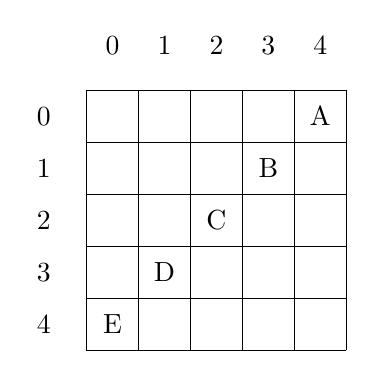
\begin{tikzpicture}[scale=0.66]
\draw (0,0) grid (5,5);
\foreach \y in {0,1,...,4} \draw(-0.5,{4.5-\y})node[left]{\y};
\foreach \x in {0,1,...,4} \draw({0.5+\x},5.5)node[above]{\x};
\draw({4.5},{4.5}) node{A};
\draw({3.5},{3.5}) node{B};
\draw({2.5},{2.5}) node{C};
\draw({1.5},{1.5}) node{D};
\draw({0.5},{0.5}) node{E};
\end{tikzpicture}}
\askN Let's represent that property:
\begin{hspec}
it "contains a diagonal made of letters" $ 
    forAll letter $ lll l ->
        let ls = ['A'..l]
            n  = length ls
            d  = diamond l
            ul = (map (take n).o.(take n)) d
            m  = n - 1
            diag j i | i == (m-j) = ul!!j!!i == ls!!j
                     | otherwise  = ul!!j!!i == ' '
        in and [diag r c | r <- [0..m], c <- [0..m]]
\end{hspec}
\answer Ok, now there is some work to do:
\begin{haskell}[frame=single]
module Diamond
where

diamond :: Char -> [String]
diamond l = map pattern [0..n]
    where 
    pattern i = (sp (n-i)) ++ [ls!!i] ++ (sp i)
    sp n = replicate n ' '
    ls = ['A'..l]
    n = length ls - 1
\end{haskell}
\askN Another interesting property of the diamond is that flipping it horizontally yields the same value.
\begin{hspec}
it "is symmetric horizontally" $ do
    forAll letter $ lll l->
        diamond l== reverse (diamond l)
\end{hspec}
\answer Indeed. Maybe we could just \il{mirror} our pattern:
\begin{haskell}[frame=single]
module Diamond
where

diamond :: Char -> [String]
diamond l = mirror (map pattern [0..n])
    where 
    pattern i = (sp (n-i)) ++ [ls!!i] ++ (sp i)
    sp n = replicate n ' '
    ls = ['A'..l]
    n = length ls - 1

    mirror xs = xs ++ reverse xs
\end{haskell}
\askN Well, guess what: flipping the diamond vertically also yields the same result.
\begin{hspec}
it "is symmetric vertically" $ do
forAll letter $ lll l->
    diamond l== map reverse (diamond l)
\end{hspec}
\answer Ok, then we will \il{mirror} each line as well. 
\begin{haskell}[frame=single]
module Diamond
where

diamond :: Char -> [String]
diamond l = mirror (map (mirror.o.pattern) [0..n])
    where 
    pattern i = (sp (n-i)) ++ [ls!!i] ++ (sp i)
    sp n = replicate n ' '
    ls = ['A'..l]
    n = length ls - 1

    mirror xs = xs ++ reverse xs
\end{haskell}
\askN Are we done with our \il{diamond} function? 
\answer Not yet: it's still lacking a property, as can be seen from this visual check: 
\begin{term}
runhaskell Main.hs D\rk
   AA
  B  B
 C    C
D      D
D      D
 C    C
  B  B
   AA
\end{term}
\askN I see. The width and height of a diamond should be an odd number. 
\begin{hspec}
it "has an odd height and width" $ do
forAll letter $ lll l ->
    odd (length (diamond l))  
    && odd (maximum (map length (diamond l)))
\end{hspec}
\answer The solution is to remove an element in the mirroring process: 
\begin{haskell}[frame=single]
module Diamond
where

diamond :: Char -> [String]
diamond l = mirror (map (mirror.o.pattern) [0..n])
    where 
    pattern i = (sp (n-i)) ++ [ls!!i] ++ (sp i)
    sp n = replicate n ' '
    ls = ['A'..l]
    n = length ls - 1

    mirror xs = xs ++ tail (reverse xs)
\end{haskell}
\askN Perfect! 
\begin{term}
runhaskell Main.hs D\rk
   A
  B B
 C   C
D     D
 C   C
  B B
   A
\end{term}
Are we done? 
\answer I don't think so. Here's a sabotaged version of the function:
\begin{haskell}[frame=single]
module Diamond
where

diamond :: Char -> [String]
diamond l = mirror (map (mir.o.pattern) [0..n])
    where 
    pattern i = (sp (n-i)) ++ [ls!!i] ++ (sp i)
    sp n = replicate n ' '
    ls = ['A'..l]
    n = length ls - 1

    mir xs = xs ++ " " ++ (tail (reverse (xs ++ " ")))
    mirror xs = xs ++ (tail (reverse xs))
\end{haskell}
Does it pass all the checks?
\askN It does. Why wouldn't that be the case?
\answer Look at what it yields: 
\begin{term}
runhaskell Main.hs D\rk
   A A
  B   B
 C     C
D       D
 C     C
  B   B
   A A
\end{term}
\askN I see. We can prevent this by adding a property that states the precise height and width of a diamond. 
\answer We know what that is: if a diamond is made with $n$ letters, then its height equals its width equals $2n-1$.
\askN Okay. Let's write a property.
\begin{hspec}
it "has an height = width = N*2-1" $ do
forAll letter $ lll l->
    let d = diamond l
        height = length d
        width  = sum (map length d) `div` height
    in height == width
    && height == length ['A'..l] * 2 - 1
\end{hspec}
\answer Ok, now the flawed version makes the checks fail. We are done.
\askN Well maybe we can refactor this code a bit. This \il{pattern} function could be improved:\\
\begin{haskell}
    pattern i = (sp (n-i)) ++ [ls!!i] ++ (sp i)
\end{haskell}
We don't need to compute each line this way. We could use list functions instead. You can try them using \emph{ghci}.\\
Try the \il{inits :: [a] -> [[a]]} function for instance.
\answer OK. 
\begin{term}
import Data.List\rk
inits "hello"\rk
["","h","he","hel","hell","hello"]
\end{term}
\askN Now write a function that given a number $n$, returns space strings of size 0,1,\dots,$n-1$.
\answer Easy: 
\begin{term}
let spaces n = take n (inits (repeat ' '))\rk
spaces 5\rk
[""," ","  ","   ","    "]
\end{term}
\askN Now using\\ \il{zipWith :: (a -> b -> c) -> [a] -> [b] -> [c]}, and \il{(:)}, you can insert each letter of the list into each space string.\\
Then you can concat that to the same space strings list, reversed.
\answer I see 
\begin{term}
zipWith (:) ['A'..'E'] (spaces 5)\rk
["A","B ","C  ","D   ","E    "]
zipWith (++) (reverse (spaces 5)) it\rk
["    A","   B ","  C  "," D   ","E    "]
Prelude Data.List> putStrLn (unlines it)\rk
    A
   B
  C
 D
E
\end{term}
I works!!
\askN Let's refactor the \il{diamond} function. 
\answer Ok. 
\begin{haskell}[frame=single]
module Diamond
where
import Data.List (inits)

diamond :: Char -> [String]
diamond l = mirror (map mirror diagonal)
    where 
    diagonal = (reverse spaces)<+>(letters<:>spaces)
    letters  = ['A'..l]
    n        = length letters
    spaces   = take n (inits (repeat ' '))
    (<+>)    = zipWith (++)
    (<:>)    = zipWith (:)
    mirror l = l ++ (tail (reverse l))
\end{haskell}
\newpage
\askN And now we are done.
\answer Let's print a big diamond. 
\begin{term}[frame=none]
runhaskell Main.hs Z\rk
                         A
                        B B
                       C   C
                      D     D
                     E       E
                    F         F
                   G           G
                  H             H
                 I               I
                J                 J
               K                   K
              L                     L
             M                       M
            N                         N
           O                           O
          P                             P
         Q                               Q
        R                                 R
       S                                   S
      T                                     T
     U                                       U
    V                                         V
   W                                           W
  X                                             X
 Y                                               Y
Z                                                 Z
 Y                                               Y
  X                                             X
   W                                           W
    V                                         V
     U                                       U
      T                                     T
       S                                   S
        R                                 R
         Q                               Q
          P                             P
           O                           O
            N                         N
             M                       M
              L                     L
               K                   K
                J                 J
                 I               I
                  H             H
                   G           G
                    F         F
                     E       E
                      D     D
                       C   C
                        B B
                         A
\end{term}
\stopasking
